\documentclass[10pt]{article}
\usepackage{../setup}
\usepackage{subfig}
\vspace{-8ex}
\date{}

\graphicspath{ {./figs/} }

\begin{document}

\title{\textbf{\Large{\textsc{ECE410:} Linear Control Systems}} \\ \Large{Lab 1 Report: Numerical Simulations of Dynamical Systems} \\ \textbf{\small{PRA102}}\vspace{-0.3cm}}
\author{Pranshu Malik, Varun Sampat \\ \footnotesize{1004138916}, \footnotesize{1003859602}\vspace{-3cm}}

\maketitle

\section{Introduction}
In this lab, we consider a pendulum-cart system with the control input, $u$, being the force imparted at the point of pivot, being the cart base, which is free to move along a frictionless rod. We consider the state of the system to be $\vec{x} = \rcvec{\theta & \dot{\theta}}$, where $\theta$ is this and has the following dynamics:

$x y$
\pendcartsimple

\section{Numerical integration Graphs and Evaluation (Section 3)}
This section models the system using the differential equations provided in the lab handout, and solves the DE by numerical integration. 

Recall, the given non-linear function was:
\begin{center}
   \begin{math}
    \dot{x} = f(x, t) = \rcvec{ x_2 \\ -\frac{g \sin x_1}{l} - \frac{\cos x_1 u(t)}{ml}}
    \end{math} 
\end{center}

There were two initial conditions of interest:
\[
\]
\begin{center}
    1.
    \begin{math}
     \vec{x}_{0,1} = \rcvec{ 0\\ \sqrt{g/l} }
    %  ;
    %  u^0_1 = 0
    \end{math}
\end{center}

\begin{center}
    2. 
    \begin{math}
     \vec{x}_{0,2} =  \rcvec{0\\1.99 \sqrt{g/l}}
    %  ;
    %  u^0_2 = 0
    \end{math}
\end{center}

Note, $x_1 = \theta$, and $x_2 = \dot{\theta}$. 
$\theta = 0$, but $\dot{\theta}$ is a non-zero value. In words, this is providing the pendulum with an initial velocity from its rest position (equilibrium at $\theta = 0$) at time $t = 0$.

$u(t) = 0$ for this section, implying the system behaves naturally; there is no forced response.

\subsection{Graphs for initial condition 1}

\begin{figure}[ht]
    \centering
    \begin{minipage}[b]{0.45\textwidth}
        \centering
        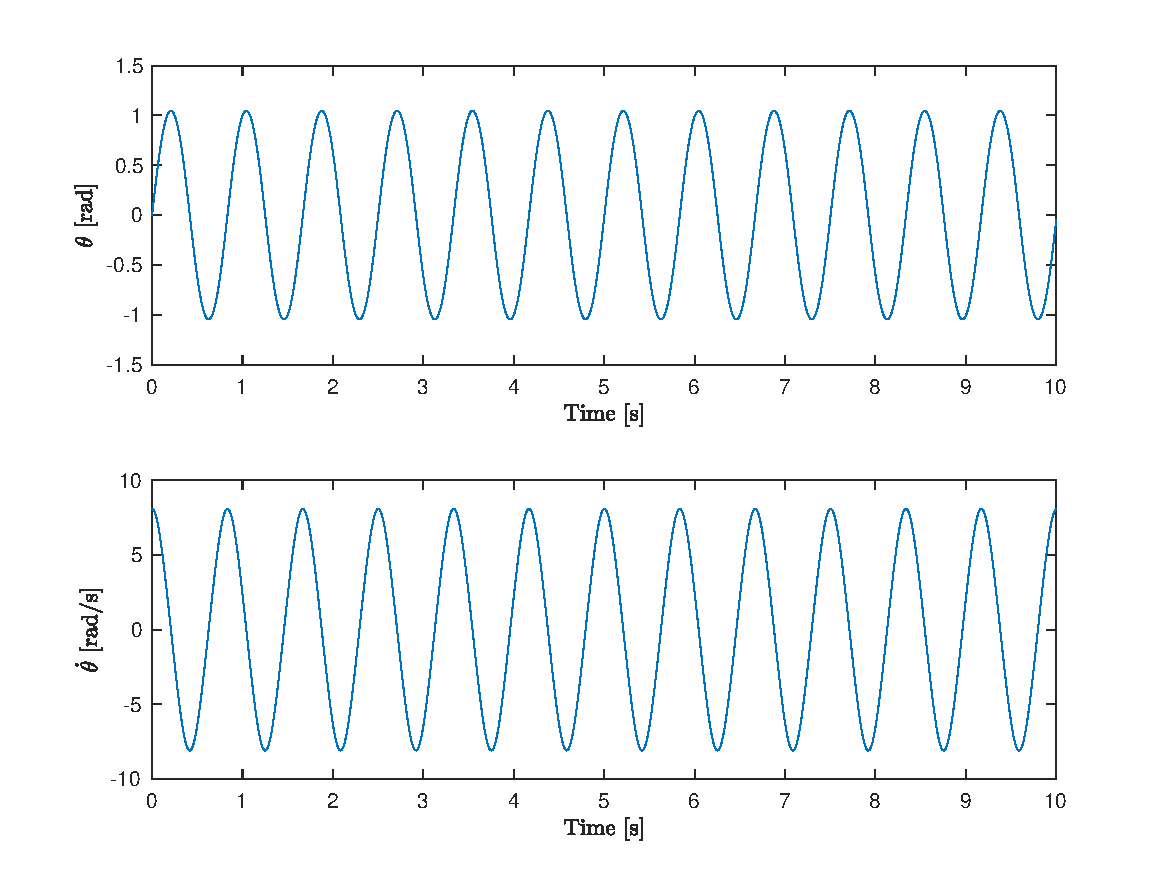
\includegraphics[width=1\linewidth]{lab1/figs/section3_x0_1_state_evolution.pdf}
        \captionof{figure}{State Evolution to initial condition 1}    
    \end{minipage}
    \begin{minipage}[b]{0.45\textwidth}
        \centering
        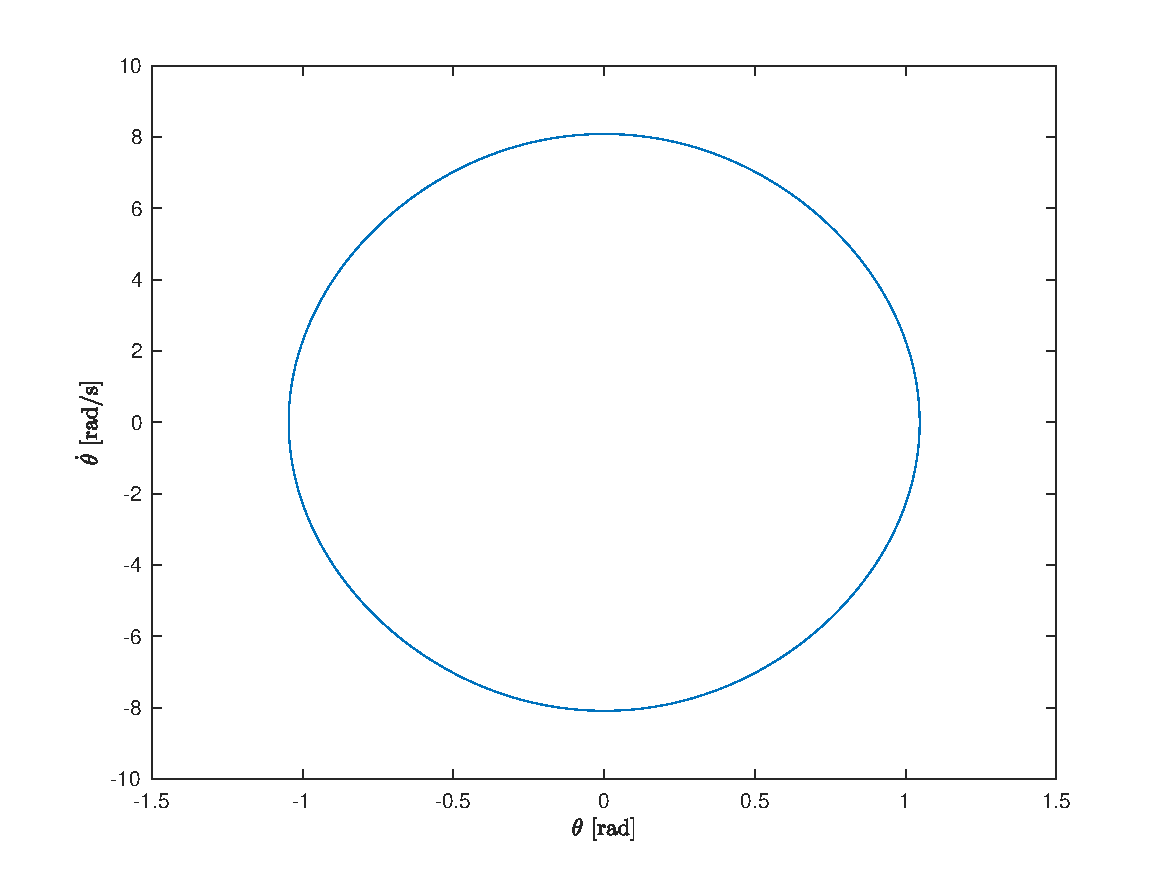
\includegraphics[width=1\linewidth]{lab1/figs/section3_x0_1_state_orbit.pdf}
        \captionof{figure}{State orbit for initial condition 1}
    \end{minipage}
    
    \label{figure:x_0_1_state_evolution}
\end{figure}
    
\subsection{Graphs for initial condition 2}
\begin{figure}[ht]
    \centering
    \begin{minipage}[b]{0.45\textwidth}
        \centering
        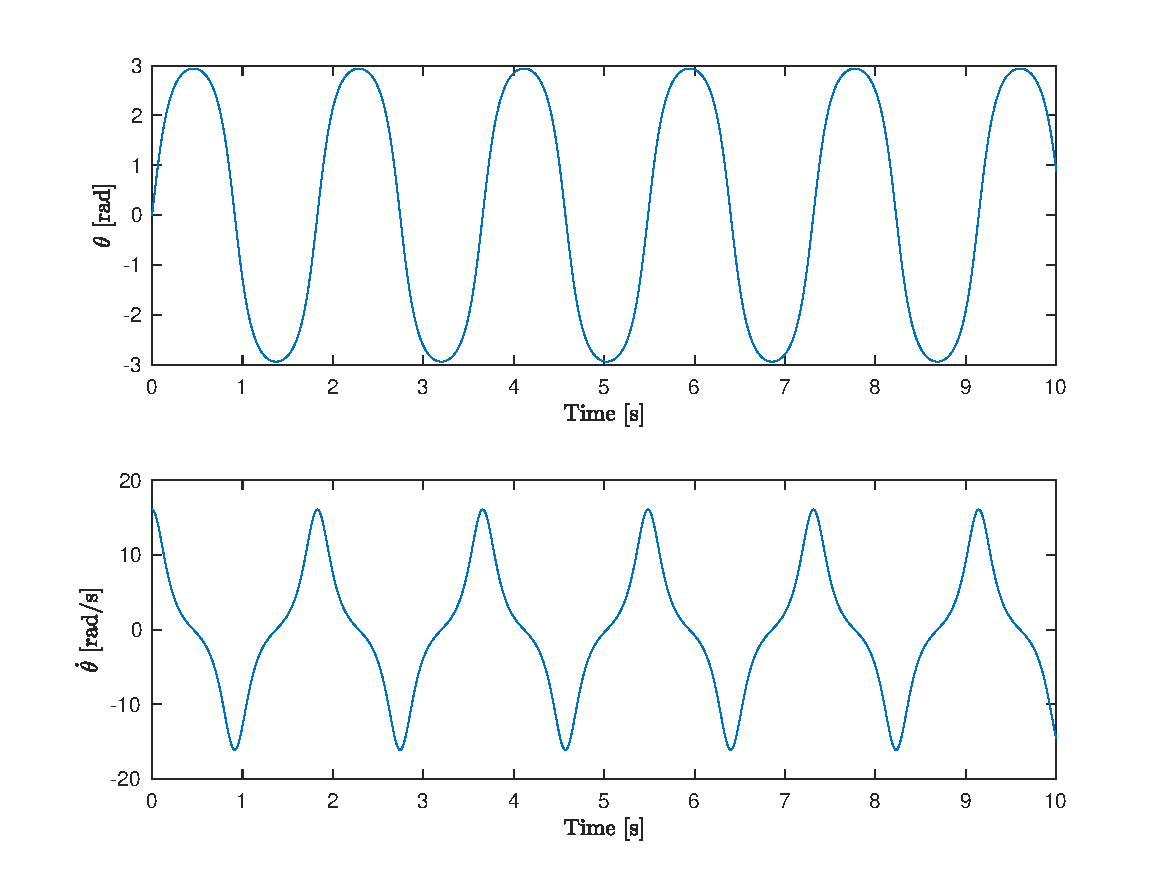
\includegraphics[width=1\linewidth]{lab1/figs/section3_x0_2_state_evolution.pdf}
        \captionof{figure}{State Evolution to initial condition 2}    
    \end{minipage}
    \begin{minipage}[b]{0.45\textwidth}
        \centering
        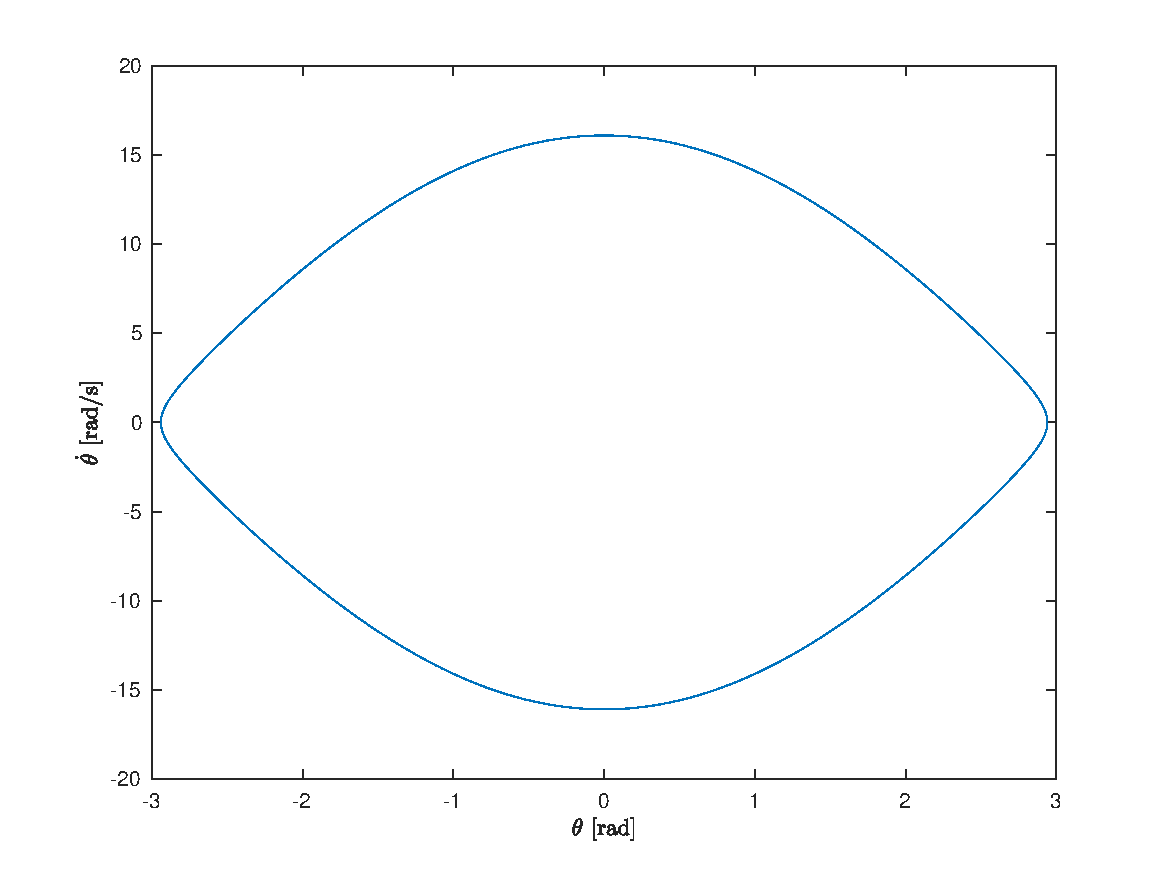
\includegraphics[width=1\linewidth]{lab1/figs/section3_x0_2_state_orbit.pdf}
        \captionof{figure}{State orbit for initial condition 2}
    \end{minipage}
    
    \label{figure:x_0_2_state_evolution}
\end{figure}

\subsection{Comparison/Analysis}
    For the first initial condition, the system response is clearly sinusoidal. For the second initial condition, however, the response is not sinusoidal. The frequency of the first initial condition is higher than the frequency of the second initial condition, on visual introspection. 
    
    To understand the difference in the responses, it is important to identify what distinguishes the initial conditions. The first condition basically injects a lower angular velocity (and hence, a lower linear velocity) than the second initial condition. Since no energy is lost here, the pendulum should sweep a higher angle for a higher initial velocity. This is seen in figures 2 and 4, where the \begin{math}
     max(\theta)_1 << max(\theta)_2
    \end{math}. Because initial condition 2 reaches a higher value of $\theta$ ($\sim$ 3 radians), one would expect a higher time period, which justifies a lower frequency than initial condition 1, that only goes up to $\sim$ 1 radian. 
    
    3 radians is $\sim$ $\pi$ which is 180 deg, which means physically speaking, the pendulum almost reaches the top. Looking at the state orbit graphs for initial condition 2, it is almost making a complete revolution; $\theta$ covered is $\sim$ -3 rad to 3 rad. A higher initial velocity would lead to the pendulum making revolutions where the same value of $\theta$ would never repeat. 
    
    Recognize that the state evolution and state orbit responses/graphs are not unique to the initial conditions for this system. For example, the first initial condition could start with $\theta$ $\sim$ 1 radian and 0 initial velocity and we would get the same system response. 
    

\section{Symbolic Linearization (Section 4)}

\subsection{Equilibrium 1}
\begin{center}
    1.
    \begin{math}
     \vec{\dot{x}} = \rcvec{0\\0}
     ;
     u = 0
    \end{math}
\end{center}

The resulting A, B matrices for this equilibrium point are:
\begin{center}
    \begin{math}
        \vec{A} = 
        \begin{bmatrix}
        0 &1 \\ \frac{-g}{l} & 0
        \end{bmatrix}
    \end{math}
    \begin{math}
        \vec{B} = 
        \begin{bmatrix}
        0\\ \frac{-1}{ml}
        \end{bmatrix}
    \end{math}
\end{center}


\subsection{Equilibrium 2}
\begin{center}
    1.
    \begin{math}
     {\dot{\vec{x}}} =
     \rcvec{\theta^* \\ 0}
     ;
     \vec{u} = -mg\tan(\theta^*)
    \end{math}
\end{center}

The resulting A, B matrices for this equilibrium point are:
\begin{center}
    \begin{math}
        \vec{A} = 
        \begin{bmatrix}
        0 &1 \\ \frac{-g\cos(\theta^*)}{l} - g \frac{\sin(\theta^*) \tan(\theta^*)}{l} & 0
        \end{bmatrix}
        =
        \begin{bmatrix}
        0 &1 \\ \frac{-g}{l\cos(\theta^*)} & 0
        \end{bmatrix}
        \end{math}
        
        (using $\tan(\theta) = \frac{\sin(\theta)}{\cos(\theta)}$)
        
        \begin{math}
        \vec{B} = 
        \begin{bmatrix}
        0\\ \frac{-\cos(\theta^*)}{ml}
        \end{bmatrix}
    \end{math}
\end{center}

The A matrix computed here matches that of the textbook. The B matrix however, contains the m (mass) term whereas the textbook has no mention of mass. If m = 1 is plugged into the equations derived above, the same equations as the textbook will be obtained. Also note, setting $\theta = 0$ here results in the same matrices derived in 3.1 ($\tan(0)$ is 0, resulting in no effect caused by the input force $\vec{u}$). 

\section{Comparing Symbolic Linearization to Numerical Integration}
Linearization was done about Equilibrium 1 defined in the previous section (3.1).

\subsection{Graphs for initial condition 1}

\begin{figure}[ht]
    \centering
    \begin{minipage}[b]{0.45\textwidth}
        \centering
        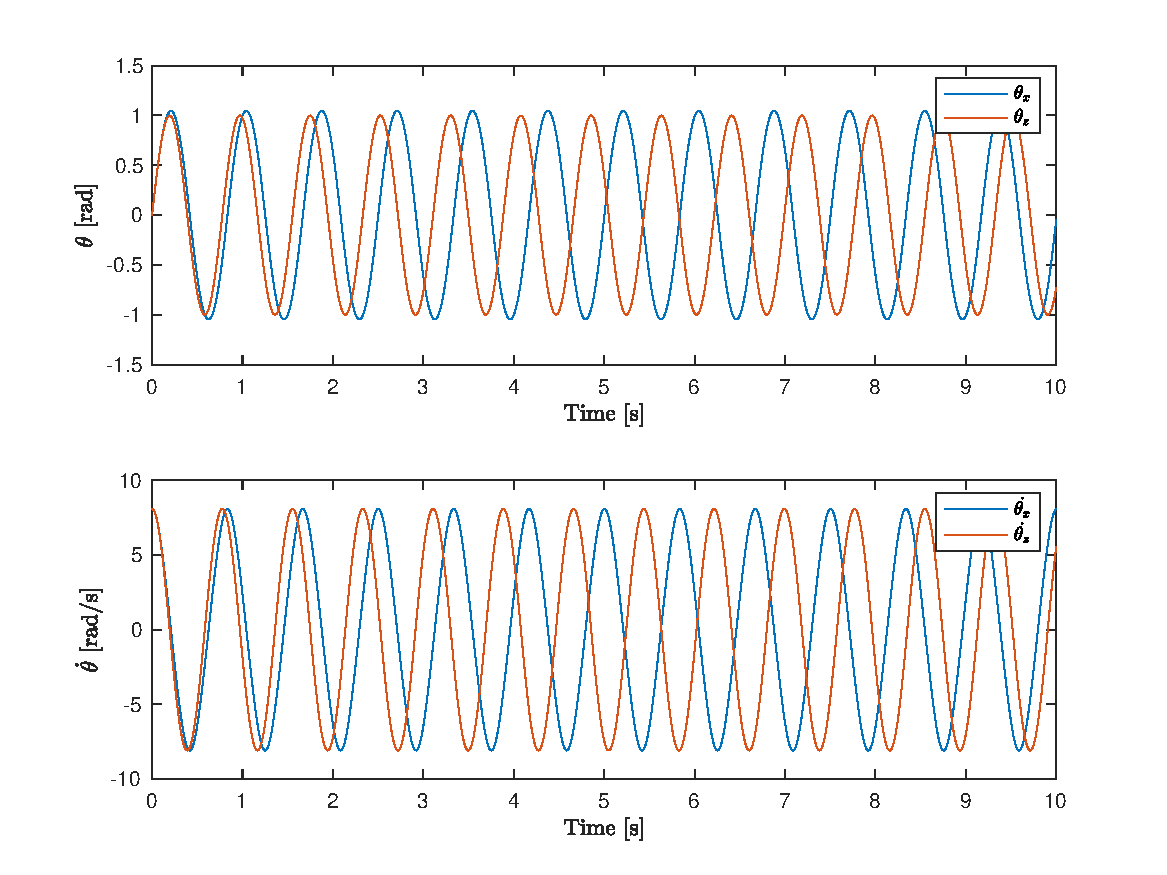
\includegraphics[width=1\linewidth]{lab1/figs/section5_X0_1_state_evolution.pdf}
        \captionof{figure}{State Evolution to initial condition 1}    
    \end{minipage}
    \begin{minipage}[b]{0.45\textwidth}
        \centering
        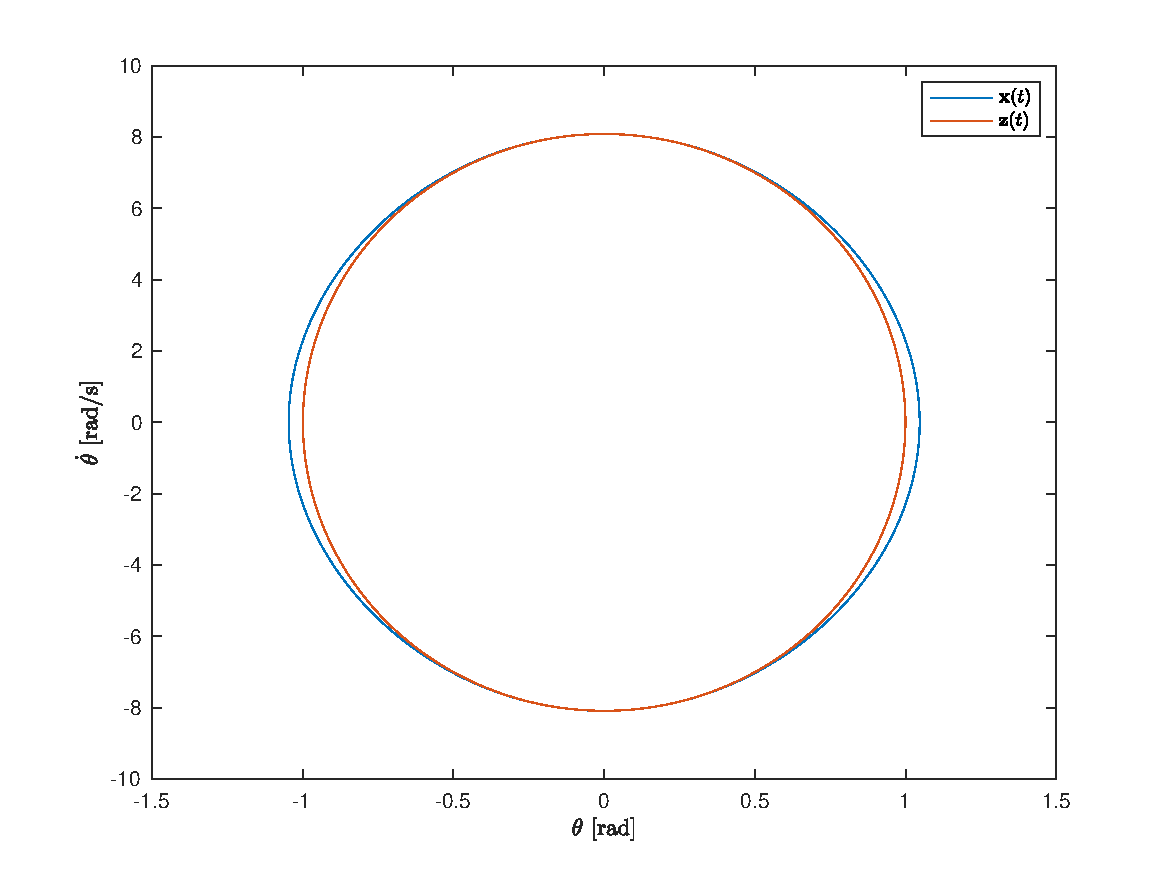
\includegraphics[width=1\linewidth]{lab1/figs/section5_X0_1_state_orbit.pdf}
        \captionof{figure}{State orbit for initial condition 1}
    \end{minipage}
    
    \label{figure:x_0_1_state_evolution}
\end{figure}
    In figure 6, it can be seen that the state space coverage is somewhat similar for the linear and non-linear models. The range for $\dot{\theta}$ is the same for the both models, but the range for $\theta$ is slightly different. The non-linear model covers an additional range at around 1 radian, which is when the linear model is not effective anymore.
    
    This additional coverage for $\theta$ is what introduces a phase shift-like  effect seen in figure 5. Both the non-linear and linear model simulations have the same initial condition, so as long as they cover the same angle, the linear model is able to follow the actual system. However, once outside of the operating region, the linear model reaches a maximum and starts heading back to the equilibrium position. In this time, the non-linear part covers an addition $\theta$ and hence starts deviating from the linear system. 
    
    % Consider $\Delta_{error} = \theta(non-linear) - \theta(linear)$, which can be obtained from the state orbit graph. While $\Delta$ is 0, the linear model will follow the actual system. 
    
    Basically, since the range for $\theta$ in the non-linear system is higher (but ever so slightly!), the frequency is ever so slightly lower than the linear model, leading to the discrepancies. A mathematical perspective that can help understand this drawback is the relationship between $f(x) = \sin(x)$ and $f(x) = x$. The linear model assumes $\sin(x) \sim x$, but this assumption is only valid at a certain range near $x \sim 0$, which explains the deviation seen in figures 5 \& 6. 
    
\subsection{Graphs for initial condition 2}
\begin{figure}[ht]
    \centering
    \begin{minipage}[b]{0.45\textwidth}
        \centering
        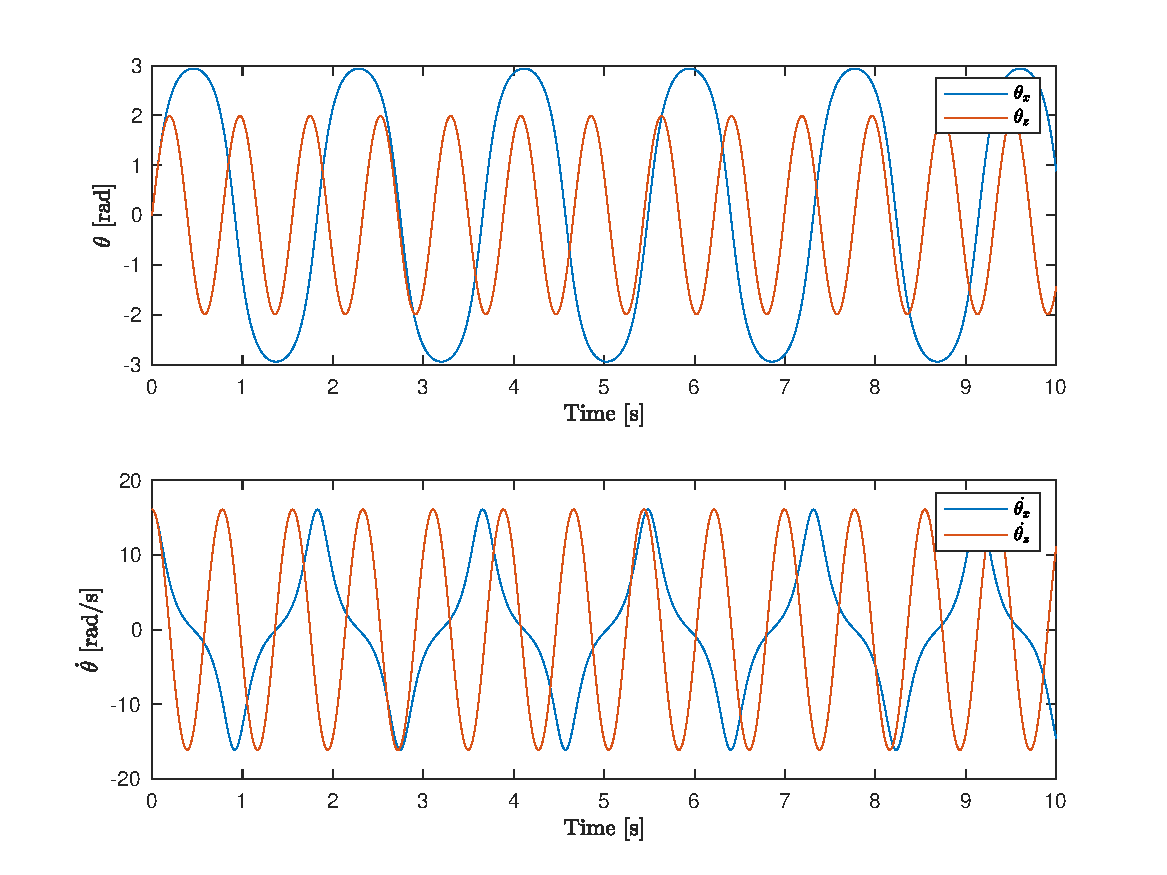
\includegraphics[width=1\linewidth]{lab1/figs/section5_X0_2_state_evolution.pdf}
        \captionof{figure}{State Evolution to initial condition 2}    
    \end{minipage}
    \begin{minipage}[b]{0.45\textwidth}
        \centering
        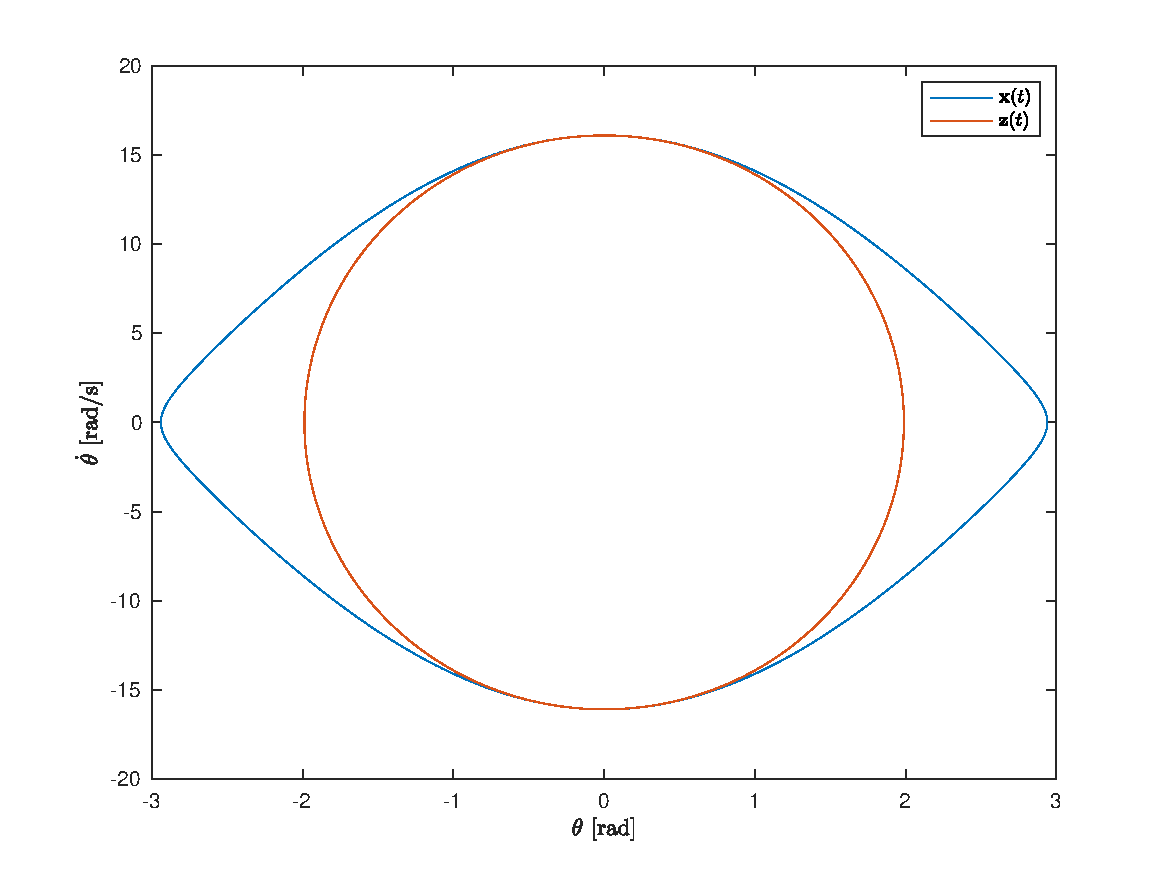
\includegraphics[width=1\linewidth]{lab1/figs/section5_X0_2_state_orbit.pdf}
        \captionof{figure}{State orbit for initial condition 2}
    \end{minipage}
    
    \label{figure:x_0_2_state_evolution}
\end{figure}
Here, the deviation talked about before is introduced earlier in the system than before. Recall that the law of conservation of energy must hold in the non-linear system, implying that every point on the state orbit has the same energy (KE + PE = constant). The linear model however, does not obey the law of conservation of energy, which explains the difference in the state orbits as well as the differences in the frequencies and amplitude. While this conflict existed in the first initial condition as well, in this condition, the differences got amplified and exposed the pitfall of the linear model.  

\subsection{Summary}
Initial condition 2 injects a higher kinetic energy than initial condition 1. This disparity led to the linear model working more accurately for initial condition 1 and observed a clear incapability to follow the system for initial condition number 2. In summary, a simple reason to explain this is that initial condition 2 reaches a higher $\theta$.

\section{Section 6: LTI Reps}
% plot eigenvalues and poles of the system!!!! Do it using pgf plots, matlab not nice for that.
Eigenvalues of A:
\begin{math}
\sigma(A) = \{8.0870i, -8.0870i\}
\end{math}

These are the eigenvectors corresponding to the given eigenvalues:
\begin{math}
    \vec{V} = \begin{bmatrix}
    -0.1227i & 0.1227i\\ 0.9924 & 0.9924 
    \end{bmatrix}
\end{math}

Transfer function of the linearized pendulum
\begin{math}
G(s) = \frac{-33.33}{s^2+65.4} = \frac{-33.33}{(s-8.0870i)(s+8.0870i)} 
\end{math}

\subsection{Analysis}
The poles of the transfer functions are the same as eigenvalues of A. This implies that there are no pole-zero cancellations taking place. Additionally, the poles are purely imaginary, implying that the system response is purely sinusoidal (no decay). This also makes sense since the differential equations that governs the system does not have any damping factor. Physcially speaking, there are no energy losses in the system, so the kinetic energy that is injected in the system infinitely oscillates between Kinetic Energy and Potential Energy. 


\subsubsection{Internal Stability}
Because the poles are purely imaginary, the system cannot be asymptotically stable. Consider $\theta = \pi/4$, then the pendulum would infinitely oscillate. However, for any starting internal state ($x_0$), the system will always produce a bounded sinusoidal output, implying that the system is stable. 


\subsubsection{Input-Output stability}
The system is also not BIBO stable as for an input force $u$ that is a sinusoidal of frequency $\sim$8.0870 rad/s (the resonance frequency), the transfer function will explode, causing to an unbounded output. This also implies that the system is not I20 stable.   
\section{Stabilization: Controller design}
\begin{math}
    C(s) = -3\frac{s+10}{10^-5s+1}
\end{math}

\begin{math}
L(s) = C(s)G(s) = \frac{100s + 1000}{10^-5s^3+s^2+0.000654s+65.4}
\end{math}

\begin{math}
1+L(s) = 1 + C(s)G(s) = \frac{(s + 9.99 \times 10^4)(s+87.97)(s+12.12)}{(s+10^5)(s^2+65.4)}
\end{math}



$\therefore$ we have something.
\mixedcls

\end{document}
